%!TEX root = ../thesis.tex
% 2 - Advanced Concepts

\chapter{Fundamental concepts about spectroscopy and RV}
\label{cha:concepts}

In this chapter the basics of \nir{} will be presented and a derivation of the of the RV equation. Following that details about the synthetic spectral models used in the work are provided. Synthetic stellar spectra {PHOENIX-ACES} and {BT-Settl} as well as atmopsheric spectra using {TAPAS}.


%!TEX root = ../../thesis.tex

NIR spectroscopy ...

Spectrograph design stuff


\section{NIR spectroscopy}
To perform spectroscopy requires an instrument called a spectrograph. The purpose of which is to take the incoming star light and disperse it so that the different wavelength components separate. A simple example of this is the splitting of white light into a rainbow when passed through a prism.

All spectrographs are comprised of a few key components.
The first part is the front end optics responsible for collecting the light and getting it to the spectrograph, such as a telescope, entrance slit or fibre.
The second part component dispersive elements inside the spectrograph, such as a prism or grating used to separate the wavelength components.
The final part is the detector or camera, used to record the resulting spectrum.

The design of spectrographs is highly dependant on the wavelength range observed. For instance {CCD} cameras (based on silicon) are readily used in the optical but silicon is a poor detector at \nir{} wavelengths.
Instead \nir{} spectrographs need to use CMOS detectors which are composed of different materials that are sensitive to different wavelengths.
{CRIRES} detectors specifically are made of \ce{InSb} (Indium antimonide) to perform spectroscopy between 1--5\um{}~\cite{dorn_crires_2004}.
Other considerations are needed such as the composition of the optical components as well as any anti-reflection coatings used, all of which have different wavelength characteristics that need to be matched.

\todo{I don't know where I am going with this section.}




%!TEX root = ../../thesis.tex


\section{Deriving the Radial Velocity}

RV derivation...
Eliptical orbit



Radial Velocity:
Picture of orbital motion.
Concepts of {RV} motion-
Masses,
Orbits, (period, mass, distance impact.)
Equation
What the Equations mean.
\begin{figure}
    \centering
    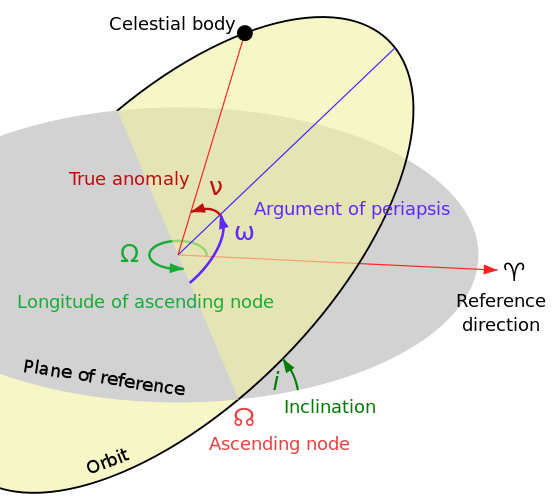
\includegraphics[width=0.5\linewidth]{figures/advanced_material/orbit}
    \caption{By Lasunncty at the English Wikipedia, CC BY-SA 3.0, \href{https://commons.wikimedia.org/w/index.php?curid=8971052}{https://commons.wikimedia.org/w/index.php?curid=8971052}}
    \label{fig:orbit}
\end{figure}


\subsection{{RV} calculation}
\unfinished{Move location / adjust from paper}
We use the Keplerian orbit {RV} equation to estimate the {RV} of the host and companions at the time of each observation, \(t\):
\begin{equation}
\label{eq:rv_equation}
{RV} = K [\cos{(\nu(t) + \omega)} + e\cos{(\omega)}]
\end{equation}
Here, \emph{K} is the \emph{semi-major amplitude}, \(\nu\) is the \emph{true anomaly}, \(e\) is the orbital \emph{eccentricity}, and \(omega\) is the \emph{argument of periastron}.
The true anomaly is not only a function time, \(t\), but also the orbital period \(P\), the \emph{time of periastron passage}, \(T_0\), and eccentricity.
The literature parameters for each target are provided in \cref{tab:orbitparams}.
To determine the {RV} of the companion we transformed the {RV} semi-amplitude of the host \(\kone\) into the semi-amplitude for the companion \(\ktwo\) using the mass ratio,
\begin{equation}
\label{eqn:mass_ratio}
q = \mtwo / \mone = \kone / \ktwo
\end{equation}

We note that for the targets in which only the minimum mass (\mtwosini) is known, this equation will indicate the maximum \(\ktwo\) value for the companion. The estimated \(\ktwo\) for each companion is provided in \cref{tab:estimatedparameters} while the {RV} for both components at the time of each observation is provided in \cref{tab:observations}.


\todo{Possibly just move this too the plae where it is used.}
The error on estimated {RV} values, shown in \cref{fig:HD211847_result_contours}, is calculated by applying the general error propagation formula~\citep{ku_notes_1966} and using the errors on the orbital parameters. For a function, \(f\), with errors on the inputs \(\delta x\), \(\delta y\) etc., it follows:
\begin{align}
f &= f(x, y, z, \ldots)\\
\delta f &= \sqrt{{\left( \frac{\partial f}{\partial x} \delta x\right)}^2 + {\left(\frac{\partial f}{\partial y} \delta y\right)}^2 + {\left(\frac{\partial f}{\partial z} \delta z\right)}^2 + \ldots}.
\end{align}




% from draft of paper 18/7/2017
\subsection{Companion K}  Maybe something can go above from this...
\label{sec:companion_RV}
\emph{These sections might be unnecessary}\\

To calculate the {RV} of the companion at the time of each observation. For a two-body system the {RV} semi-amplitude of the companion \(\ktwo\) can be determined from the orbital host-companion mass ratio
\begin{equation}
q = \mone/\mtwo = \ktwo/\kone\label{eqn:q_ratio_K2}.
\end{equation}
Note, that for the targets in which only the minimum mass (\mtwosini) is known, this will give the maximum {RV} semi-amplitude of the companion.
This relation was used to estimate \(\ktwo\) for the companion from the minimum mass or mass we have for each companion. These values along with the other orbital parameters of the system were used to calculate the {RV} of the companions for each observation. These values are provided with the observations in \cref{tab:observations}.




If more than one planet is present then they gravitational influence each other and their orbits become non-Keplerian, i.e.\ a N-body problem? {\textbf{ref}}. In this work were a star has two companions we will only assume Keplerian orbits from individual planets, independently.




\section{Estimating Companion-host Flux ratio}
\label{sec:compaion_flux_ratio}
In order to visually or spectroscopically detect binary or planetary companions it is helpful to calculate the flux/contrast ratio between the host and companion.

The companion-host flux or contrast ratio of the system can be estimated using:
\begin{equation}
\frac{F_{2}}{F_{1}} \approx 2.512^{m_{1} - m_{2}}, \label{eqn:mag_flux_ratios}
\end{equation}
where \(m_{1}\) and \(m_{2}\) are the magnitude of the host and companion respectively.

The photometric apparent magnitudes for the host stars, \(m_{1}\), in several wavelength bands are easily obtained through online catalogues such as {SIMBAD}~\citep{wenger_simbad_2000} or {2MASS} \citep{skrutskie_two_2006}.
However, the magnitudes of the companions, \(m_{2}\), are not readily available as they have not been directly measured.
Stellar evolution models of \citet{baraffe_evolutionary_2003, baraffe_new_2015} are used to estimate the magnitude of the companion.
These models tabulate several properties of low-mass stars and BDs during their evolution.
These include the temperature, radius, luminosity, and absolute magnitudes in several photometric bands, for a range of companion masses and stellar ages.
A given companion mass, and a stellar age will uniquely identify a point in the Baraffe models which corresponds to a specific magnitude for the companion.
The tables provided in \citet{baraffe_evolutionary_2003, baraffe_new_2015} are also interpolated to reach companion masses and stellar ages between the models provided.

In \cref{tab:estimated_flux_ratios} the host-companion flux ratio estimates for the targets analysed in this work are presented. The {K}-band flux ratios are calculated to match the observed {CRIRES} spectra at 2.1\um{}. The stellar ages used for the each system are given in \cref{tab:starparams} while the companion masses are given from \cref{tab:orbitparams}. The age and companion mass are both used to obtain the absolute magnitude for the companions. For the companions in which only the minimum mass (\mtwosini{}) is known then the flux-ratio given will be the lower limit, or worst case scenario.

%!TEX root = ../../thesis.tex
\begin{table*}
    \small
    \centering
    \begin{threeparttable}[b]
        \caption{Estimated flux ratios given the companion mass (\(\textrm{M}_{2}\) or \(\textrm{M}_{2} \sin{i}\)) from \tref{tab:orbitparams}.} 
        \begin{tabular}{l c c c c c c}%[hb]
            \toprule
            & Host& & Host & Companion & Estimated & Estimated  \\  % 2017
            Companion & $m_{K}$ & $\pi$ & M\(_{K}\) & M\(_{K}\) & \(\rm F_{2}/F_{1} \) & \(\rm N_{2}/N_{1} \) \\
            & & mas & & & \textit{K}-band &  (noise ratio) \\
            \midrule
            {HD 4747} & 5.305 & 53.184 & 3.82 & 14.17 & \(7\times10^{-5} \) & 76 \\  % 2017
            {HD 162020} & 6.539 & 32.410 & 4.10 & 23.36 & \(2\times10^{-8} \) & 1\,615 \\  %
            {HD 167665} & 5.038 & 32.014 & 2.60 & 13.21 & \(6\times10^{-5} \) & 105 \\  %  -- \(2\times10^{-5} \)  best case based on age rage.
            {HD 168443b} & 5.211 & 25.208 & 2.35 & 42.19 & \(1\times10^{-16} \) & \(1\times10^{8} \) \\ 
            {HD 168443c} & 5.211 & 25.208 & 2.35 & 29.55 & \(1\times10^{-11} \) & \(4\times10^{5} \) \\  %(c)
            {HD 202206}B & 6.485\tnote{a}& 21.726 & 3.04 & 21.63 & \(4\times10^{-8} \) & 1\,586 \\  %(B)   % May2017
            {HD 202206}c & 6.485\tnote{a}& 21.726 & 3.04 & 45.63 & \(9\times10^{-18}\) & \(2\times10^{7} \) \\  %(B)   % May2017
            {HD 211847}B & 7.018 & 20.489 & 3.50 & 8.40 & 0.011 & 14 \\  %B % 2017
            {HD 30501} & 5.525 & 49.081 & 3.96 & 10.38 & 0.003 & 27 \\
            \bottomrule
        \end{tabular}\label{tab:estimated_flux_ratios}
        \begin{tablenotes}
            \item  [a]{Magnitude from {2MASS} catalogue instead of {SIMBAD}.}
        \end{tablenotes}
    \end{threeparttable}

\end{table*} % \label{tab:estimated_flux_ratios}

The magnitudes provided by {SIMBAD} are given in apparent magnitude, $m$, while the magnitudes in the evolutionary models are absolute magnitudes $M$. That is, the apparent magnitude that the star would have if it was observed at a distance of 10 parsecs (32.6 light-years). The apparent magnitudes of the hosts are converted to absolute magnitudes using \(M = m - \mu\) where \(\mu\) is the distance modulus:
\begin{equation}
\mu = 5 \log_{10}(d_{pc}) -5. \label{eqn:distance_modulus}
\end{equation}
Here $d_{pc}$ is the distance to the object in parsec. The distance is obtained from the trigonometric parallax  $\pi$ using the formula $d(pc) = 1 /\pi(arcsec)$, with the parallax in arcseconds\footnote{Most parallax values e.g.\ GAIA are tabulated in milliarcseconds (mas). Therefore it is important to remember to convert the parallax to arcseconds first, to avoid embarrassing calculation errors!}. In this work the recent high-precision parallax measurements from GAIA are used~\citet{collaboration_gaia_2018}.

From the flux ratio the noise ratio between the host and companion can also be calculated in a similar way using the equation \(N_{2}/N_{1} = \sqrt{2} \times\sqrt{F_{1}/F_{2}}\).

\todo{this section is completed i think}

\subsubsection{Baraffe tables}
\label{subsubsec:baraffe_tables_code}
A simple tool\footnote{Available at \url{https://github.com/jason-neal/baraffe_tables}} was created to calculate/estimate the host-companion flux ratio using the \citet{baraffe_evolutionary_2003,baraffe_new_2015} evolution tables.
Given the name of the target star, the mass of a companion and the stellar/system age the tool determines the flux ratios in the available spectral bands.
The tool uses the targets name to query\href{https://zenodo.org/record/1160627}{\emph{astroquery} package} the {SIMBAD} database to obtain the stellar properties, specifically the flux magnitudes and parallax. It then interpolates the Baraffe tables to the desired companion mass and age, calculating and returning values for all parameters of the companion given in the tables (e.g.\ \(\teff\), \logg, \(R/R_{\odot}\)).
The stellar magnitudes are converted to absolute values using \cref{eqn:distance_modulus} and the flux ratios computed using  \cref{eqn:mag_flux_ratios}.

An extension of this tool is that can be used to perform the reverse calculation also. That is, given the target name, age and flux ratio in a given band it can estimate the mass of the companion mass using the Baraffe tables.

\todo{This section is completed I think}


%!TEX root = ../../thesis.tex


\section{Telluric correction}


\subsection{Telluric models}

Utilizing telluric models has been shown to be better than the standard star method.
\subsubsection{TAPAS}

\subsection{Tapas models}
\todo{ADAPT THis section to explain the models more generally. Move the usage back to Reduction section}
\label{subsec:tapas_models}
For the wavelength calibration and telluric correction methods we use telluric line models. These have been show to provide as good or better telluric correction compared to the telluric standard method \reference{telluric model correction methods original}and~\citep{ulmer-moll_telluric_2018}.

We utilized the {TAPAS} (Transmissions of the AtmosPhere for AStronomical data) web-service\footnote{\url{http://www.pole-ether.fr/tapas/}}~\citep{bertaux_tapas_2014} to obtain atmospheric transmission models for each observation. {TAPAS} uses the standard line-by-line radiative transfer model code LBLRTM~\citep{clough_linebyline_1995} along with the 2008 {HITRAN} spectroscopic database~\citep{rothman_hitran_2009} and {ARLETTY} atmospheric profiles derived using meteorological measurements from the {ETHER} data center\footnote{\url{http://www.pole-ether.fr}} to create telluric line models.

The {ARLETTY} atmospheric profiles have a 6 hour resolution, so there may be a slight difference between the actual profile at the time of observation.

We use the mid-observation time to retrieve transmission models for each observation, with the {ARLETTY} atmospheric profiles\footnote{Nearest of the 6 hourly profiles} and vacuum wavelengths selected. The telluric models were retrieved without any barycentric correction to keep the telluric lines at a radial velocity of zero with respect to the instrument.

{TAPAS} allows for the choice of atmospheric constituents included in the model spectra. We obtained one model with all available species present, convolved to a resolution of \(\rm R=50\,000\), and another two models without an instrumental profile convolution applied. For these two extra models, one contained only the transmission spectra of \ce{H2O} while the other contained all other constituents except \ce{H2O}. This was to explore a known issue with the depth of \ce{H2O} absorption lines in the TAPAS~\citet{bertaux_tapas_2014}. \sref{subsec:telluric_correction}.


\todo{Look at} -> synthesizing telluric spectra \nir{} for {CRIRES}~\cite{seifahrt_synthesising_2010}

Using {TAPAS} is contrasted alongside Molecfit and Telfit in~\cite{ulmer-moll_telluric_2018}. We conclude that \ldots





%!TEX root = ../../thesis.tex

\section{Synthetic Stellar models}:

In the work we make extensive use of the {PHOENIX-ACES} models with some experimentation with the {BT-Settl} models.
A collection of several theoretical stellar spectral libraries can be found at Spanish Virtual Observatory \href{http://svo2.cab.inta-csic.es/theory/newov/index.php}{Theoretical Spectra Web Server}.



\subsection{PHOENIX-ACES}

Available \todo{FINISH}




\subsection{BT-Settl}

Available \todo{FINISH}

Harder to work with.

Other models which have not been used here.
Kruz models a directory of different model can be found \ldots{}?

BT-Settl have less but are ore suitable for BD.
We did not extend below the {PHOENIX-ACES} lower temperature of 2300\K{}




\subsection{Differential techniques}
\todo{maybe this should go in differential chapter}
See \citet{kostogryz_spectral_2013} for lots of useful references regarding differential works \citet{simon_disentangling_1994}

\citet{rodler_weighing_2012} uses differential of a series of phases to construct a stellar mask for the host to subtract from all measurements.
